\documentclass{beamer}
\usetheme{Warsaw}  %% Themenwahl

\usepackage[utf8]{inputenc}
\usepackage[ngerman]{babel}
\usepackage{ngerman}
 
\title{Komponenten von SHA256}
\author{Lars Schmertmann}
\date{\today}
 
\begin{document}
\maketitle
\frame{\tableofcontents[currentsection]}
 
\section{Komponenten}
\subsection{Padding}
  \begin{frame}
    \frametitle{Padding}
    Auffüllen der Eingabe auf ein Vielfaches von 512 Bit.\\
    ~\\
    Allgemeines Padding:\\
    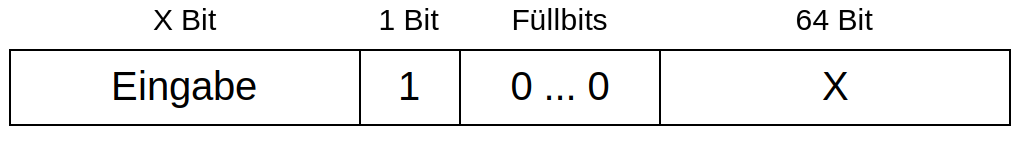
\includegraphics[width=300pt]{padding.pdf}\\
    \pause~\\
    Mögliche Lösung für SAT-Berechnung\\
    - Länge von 55 Byte vorgeben:\\
    \includegraphics[width=300pt]{padding-allgemein.pdf}
  \end{frame}
\subsection{Funktionen}
  \begin{frame}
    \frametitle{Funktionen}
    \begin{itemize}
      \setlength{\itemsep}{20pt}
      \item Expansion
        \begin{itemize}
          \setlength{\itemsep}{10pt}
          \item $ SSIG0(x) = ROTR^{7}(x)~XOR~ROTR^{18}(x)~XOR~SHR^{3}(x) $
          \item $ SSIG1(x) = ROTR^{17}(x)~XOR~ROTR^{19}(x)~XOR~SHR^{10}(x) $
        \end{itemize}
      \item Computation
        \begin{itemize}
          \setlength{\itemsep}{10pt}
          \item $ CH( x, y, z) = (x~AND~y)~XOR~( (NOT~x)~AND~z) $
          \item $ MAJ( x, y, z) = (x~AND~y)~XOR~(x~AND~z)~XOR~(y~AND~z) $
          \item $ BSIG0(x) = ROTR^{2}(x)~XOR~ROTR^{13}(x)~XOR~ROTR^{22}(x) $
          \item $ BSIG1(x) = ROTR^{6}(x)~XOR~ROTR^{11}(x)~XOR~ROTR^{25}(x) $
        \end{itemize}
    \end{itemize}
  \end{frame}
\subsection{Expansion}
  \begin{frame}
    \frametitle{Expansion}
    Jeder Block der Länge 512 Bit wird auf 2048 Bit erweitert.\\
    ~\\
    Die zusätzliche Bits werden wie folgt generiert:\\
    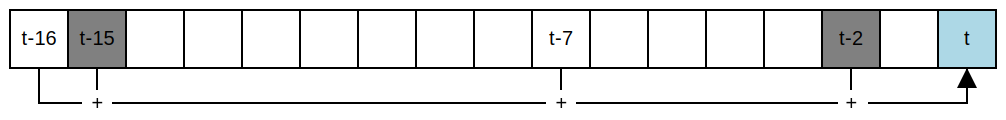
\includegraphics[width=300pt]{extend.pdf}
  \end{frame}
\subsection{Computation}
  \begin{frame}
    \frametitle{Computation}
    \includegraphics[width=300pt]{sha256.pdf}
  \end{frame}

\section{Bitcoin}
\subsection{Aufgabe}
  \begin{frame}
    \frametitle{Aufgabe}
    Aufbau eines Bitcoinblocks:
    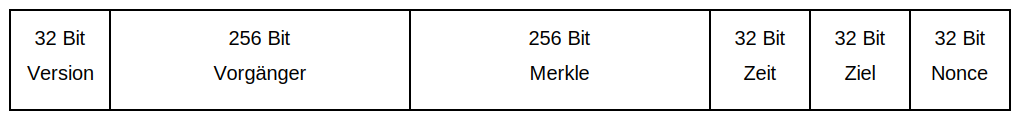
\includegraphics[width=300pt]{bitcoinblock.pdf}\\
    ~\\
    Aufgabe:\\
    Finde eine Nonce, so dass SHA256(SHA256(Block))\\
    kleiner als das aktuelle Ziel ist.\\
    ~\\
    Das bedeutet aktuell:\\
    Der Hashwert muss 67 führende Nullen haben.
  \end{frame}
\subsection{Padding}
  \begin{frame}
    \frametitle{Padding}
    Eingabe für die erste Hashberechnung:
    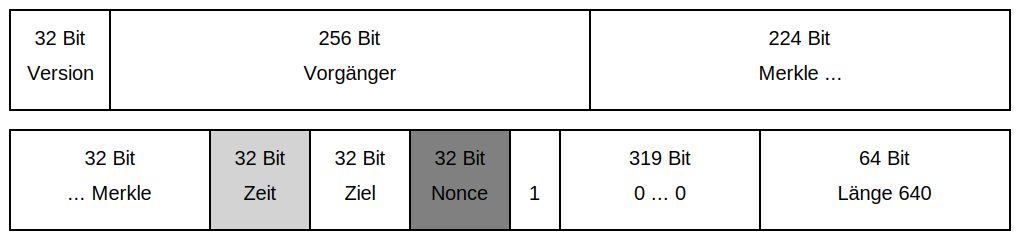
\includegraphics[width=300pt]{blockpadding.pdf}\\
    ~\\
    Eingabe für die zweite Hashberechnung:
    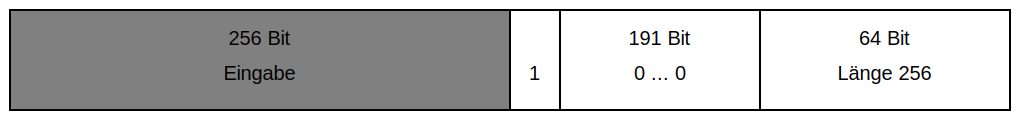
\includegraphics[width=300pt]{blockpadding2.pdf}\\
  \end{frame}
\end{document}